%% LyX 2.3.7 created this file.  For more info, see http://www.lyx.org/.
%% Do not edit unless you really know what you are doing.
\documentclass[english]{article}
\usepackage[T1]{fontenc}
\usepackage[latin9]{inputenc}
\usepackage{array}
\usepackage{float}
\usepackage{url}
\usepackage{amssymb}
\usepackage{graphicx}

\makeatletter

%%%%%%%%%%%%%%%%%%%%%%%%%%%%%% LyX specific LaTeX commands.
%% Because html converters don't know tabularnewline
\providecommand{\tabularnewline}{\\}

%%%%%%%%%%%%%%%%%%%%%%%%%%%%%% Textclass specific LaTeX commands.
\newenvironment{lyxcode}
	{\par\begin{list}{}{
		\setlength{\rightmargin}{\leftmargin}
		\setlength{\listparindent}{0pt}% needed for AMS classes
		\raggedright
		\setlength{\itemsep}{0pt}
		\setlength{\parsep}{0pt}
		\normalfont\ttfamily}%
	 \item[]}
	{\end{list}}

\makeatother

\usepackage{babel}
\usepackage{listings}
\renewcommand{\lstlistingname}{Listing}

\begin{document}
\title{OPTIMUS: a multidimensional global optimization package}
\author{Ioannis G. Tsoulos$^{(1)}$\thanks{corresponding author. Email: itsoulos@uoi.gr},
Vasileios Charilogis$^{(1)}$, V.N. Stavrou$^{(2)}$,Alexandros Tzallas$^{(1)}$ }
\date{$^{1}$\quad{}Department of Informatics and Telecommunications, University
of Ioannina\\
$^{2}\quad$Division of Physical Sciences, Hellenic Naval Academy,
Military Institutions of University Education, 18539 Piraeus, Greece}
\maketitle
\begin{abstract}
A significant number of applications from many research areas can
be considered global optimization problems, such as applications in
the area of image processing, medical informatics, economic models,
etc. This paper presents a programming tool written in ANSI C++, which
researchers can use to formulate the problem to be solved and then
make use of the local and global optimization methods provided by
this tool to efficiently solve such problems. The main features of
the suggested software are: a) Coding of the objective problem in
a high level language such as ANSI C++ b) Incorporation of many global
optimization techniques to tackle the objective problem c)Parameterization
of global optimization methods using user-defined parameters.
\end{abstract}
\textbf{PACS}:02.60.-x ; 02.60.Pn ; 07.05.Kf;  02.70.Lq; 07.05.Mh 

\section*{PROGRAM SUMMARY }

\textit{Title of program}: Optimus

\textit{Catalogue identifier}:

\begin{flushleft}
\textit{Program available from}: CPC Program Library, Queen's University
of Belfast, N. Ireland.
\par\end{flushleft}

\begin{flushleft}
\textit{Computer for which the program is designed and others on which
it has been tested}: The tool has been tested on Linux, Windows and
FreeBSD. The tool is designed to be portable in all systems running
the GNU C++ compiler and the freely available library of QT. Also,
some methods can use the freely available library of OpenMP for parallelization.
\par\end{flushleft}

\begin{flushleft}
\emph{Installation}: University of Ioannina, Greece.
\par\end{flushleft}

\begin{flushleft}
\textit{Programming language used}: GNU-C++.
\par\end{flushleft}

\begin{flushleft}
\emph{Memory required to execute with typical data}: 200KB.
\par\end{flushleft}

\begin{flushleft}
\textit{No. of bits in a word}: 64
\par\end{flushleft}

\begin{flushleft}
\emph{No. of processors used}: many
\par\end{flushleft}

\begin{flushleft}
\emph{Has the code been vectorized or parallelized?}: Yes, using the
OpenMP library.
\par\end{flushleft}

\begin{flushleft}
\emph{No. of bytes in distributed program,including test data etc}.:
100 Kbytes.
\par\end{flushleft}

\begin{flushleft}
\emph{Distribution format}: gzipped tar file.
\par\end{flushleft}

\begin{flushleft}
\emph{Keywords}: Global optimization, stochastic methods.
\par\end{flushleft}

\begin{flushleft}
\emph{Nature of physical problem}: A series of problems in science
and engineering usually can be formulated as a problem of minimizing
a function of many variables. The so called local optimization techniques
are frequently trapped in local minima, that it sub optimal solutions.
For that reason researchers should use more advanced methods that
aim to estimate the global minimum of the function.
\par\end{flushleft}

\begin{flushleft}
\emph{Typical running time}: Depending on the objective function.
\par\end{flushleft}

\section*{LONG WRITE UP}

\section{Introduction }

The location of the global minimum for a continuous and differentiable
function $f:S\rightarrow R,S\subset R^{n}$ is formulated as
\begin{equation}
x^{*}=\mbox{arg}\min_{x\in S}f(x)\label{eq:eq1}
\end{equation}
where the set $S$ is defined as: 
\[
S=\left[a_{1},b_{1}\right]\otimes\left[a_{2},b_{2}\right]\otimes\ldots\left[a_{n},b_{n}\right]
\]
Methods that aim to locate the global minimum finds application in
problems from the area of economics \cite{globalecon1,globalecon2},
problems that appear very often in the area of physics \cite{global_physics1,global_physics2},
chemistry \cite{global_chemistry1,global_chemistry2}, common problems
from medicine \cite{global_med1,global_med2}, job scheduling problems
\cite{global_job1,global_job2}, water resources planning \cite{global_water1,global_water2},
network security problems \cite{global_network1,global_network2},
robotics \cite{global_robot1,global_robot2} etc. Also, global optimization
methods were used on some symmetry problems \cite{go_symmetry0,go_symmetry1,go_symmetry2}
as well as on inverse problems \cite{global_nonlinear1,global_nonlinear2,global_nonlinear3}.
In the relevant literature there are a number of global optimization
techniques, such as Adaptive Random Search methods \cite{go_adaptive1,go_adaptive2},
Controlled Random Search methods \cite{go_crs1,go_crs2}, Simulated
Annealing \cite{go_sa1,go_sa2,go_sa3}, Genetic algorithms \cite{go_ga1,go_ga2},
Ant Colony Optimization \cite{go_ant1,go_ant2}, Particle Swarm Optimization
\cite{go_pso1,go_pso2} etc. 

Due to the high importance of the global optimization problem, a variety
of hybrid optimization techniques have been proposed to handle the
global optimization problem, such as methods that combine Particle
Swarm Optimization and Genetic algorithms \cite{go_pso_genetic_hybrid1,go_pso_genetic_hybrid2},
combination of genetic algorithms and fuzzy logic classifier \cite{ga_fuzzy},
incorporation of genetic algorithm and the K-Means algorithm \cite{ga_kmeans},
combination of Particle Swarm Optimization method with Ant Colony
Optimization \cite{pso_aco1,pso_aco2,pso_aco3}, methods that combine
the Simplex method and Inductive search \cite{hybrid1} etc. Also,
many hybrid techniques combining local and global optimization have
been developed \cite{go_local1,go_local2,go_local3}.

Just a few recent application examples include an adaptive genetic
algorithm for crystal structure prediction \cite{genetic_physics1},
modeling of fusion plasma physics with genetic algorithms \cite{genetic_physics2},
usage of genetic algorithms for astroparticle physics studies \cite{genetic_physics3},
parameter extraction of solar cells using a Particle Swarm Optimization
method \cite{pso_physics1}, a new control approach of a a fleet of
Unmanned Aerial Vehicles using the method of Particle Swarm Optimization\cite{pso_physics2}
etc.

However, in most cases, global optimization methods require a lot
of computing resources to implement both in memory and computing time.
Because of the large demands that global optimization methods have
on computing power, several techniques have been proposed, such as
asynchronous methods \cite{async1,async2,async3}, parallel approaches
of the Multistart optimization method \cite{parallel-multistart,parallel-multistart2}
and also some methods that take advantage of modern parallel GPU architectures
\cite{gpu1,gpu2,gpu3}.

In this paper, a new integrated computing environment for performing
global optimization methods for multidimensional functions is presented
and analyzed in detail. In this computing environment, the programmer
can code the problem to be solved using a high-level programming language
such as C++. In addition to the objective function, the programmer
can also provide information that the objective problem should have
at the start of the optimization process and, in addition, can formulate
a series of actions that will take place after the optimization process
is finished. Subsequently, the researcher can formulate a strategy
to solve the problem. In this strategy, the researcher can choose
from a series of sampling methods, choose a global minimization method
established in the relevant literature and possibly some local minimization
method to improve the produced result. Similar software environments
can be found, such as the BARON software package \cite{baron} for
non-convex optimization problems, the MERLIN optimization software
\cite{merlin} which is accompanied by the Merlin Control Language
compiler to guide the optimization course, the DEoptim software \cite{deoptim}
which is an R package implementing the differential evolution algorithm,
the PDoublePop optimization software \cite{pdoublepop} that implements
a parallel genetic algorithm for global optimization etc.

Also recently, some other optimization tools have appeared such as
the Paradiseo \cite{paradiseo} implemented in C++, which mainly includes
evolutionary algorithms, the Pagmo software \cite{pagmo} where a
wide range of evolution algorithms are incorporated to solve optimization
problems, and finally another approach for evolutionary algorithms
applied to optimization problems is the HeuristicLab freely available
from \url{https://dev.heuristiclab.com/trac.fcgi/}, used mainly for
online optimization. In the proposed software, the user can write
the required objective function in simple C++ and then choose from
a wide range of global optimization methods, the most suitable one
for finding the global minimum. Furthermore, in the proposed software,
the user can parameterize the local minimization method to be used
as well as the termination method to be used for the successful termination
of the technique. In addition, it is possible for the user to create
his own global minimization method from scratch using the programming
tools of the Optimus libraries.

The rest of this article is structured as follows: in section \ref{sec:Software}
the proposed software is outlined in detail, in section \ref{sec:Experiments}
some experiments are conducted to show the effectiveness of the proposed
software and finally in section \ref{sec:Conclusions} some conclusions
and guidelines for future work are presented.

\section{Software\label{sec:Software}}

The suggested software is entirely coded in ANSI C++, using the freely
available QT programming library, which can be downloaded from \url{https://qt.io}
(accessed on 8 February 2023). The researcher should code the objective
function and a number of other mandatory functions in the C++ programming
language. Also, the researcher should provide the dimension of the
objective function as well as the bound of the function (equation
\ref{eq:eq1}). Subsequently, the user can select a global optimization
method to apply to the problem from a wide range of available methods.
Also, the user can extend the series of methods by adding any new
method that follows the guidelines of the software.\textbf{ }In the
following subsections, the installation process of the suggested software
will be analyzed and a complete example of running an objective problem
will be given.

\subsection{Installation }

The software can be installed in almost any operating system running
a C++ compiler and the freely available library of QT. The steps to
install the software are similar to most operating systems and have
as follows:
\begin{enumerate}
\item Download and install the QT programming library from \url{https://qt.io }. 
\item Download and unzip the software from \url{https://github.com/itsoulos/GlobalOptimus}.
\item Issue the command:\emph{ cd GlobalOptimus-master }
\item Execute the command \emph{qmake} (or \emph{qmake-qt5} in some installations).
\item Execute the command \emph{make}
\end{enumerate}
The compilation will take some minutes and the final outcome of this
compilation will be the executable \emph{GlobalOptimus}.

\subsection{Implemented global optimization methods }

In the following, the global optimization methods present in the proposed
software are presented. In most of them, a local optimization method
is applied after their end in order to find the global minimum with
greater reliability. In the proposed software, each implemented global
optimization method has a set of parameters that can determine the
global optimization path and the effectiveness of the method. For
example, the genetic algorithm contains parameters such as the number
of chromosomes or the maximum number of generations allowed. In addition,
to make the optimization process easier, each method has been assigned
a symbolic name, such as pso for particle swarm optimization. The
implemented global optimization methods are:
\begin{enumerate}
\item Differential Evolution. The differential evolution method is included
in the software as suggested by Storn\cite{de_main_paper} and denoted
as \textbf{DifferentialEvolution}. This global optimization technique
has been widely used in areas such as data mining applications \cite{de_datamining,de_symmetry1},
material design problems \cite{de_symmetry3}, feature selection \cite{de_symmetry6},
clustering methods \cite{de_symmetry7} etc.\textbf{ }
\item Parallel Differential Evolution. A parallel implementation of the
Differential Evolution method as suggested in \cite{parallelDe} is
considered with the name \textbf{ParallelDe}. This parallel technique
divides the total work into a number of available parallel computing
units, and in each unit an independent Differential Evolution method
is executed. The parallelization is done using the OpenMP programming
library \cite{openMp}.
\item Double precision genetic algorithm. A modified genetic algorithm \cite{doublepop_tsoulos}
is included in the software and it is denoted as \textbf{Genetic}.
Genetic algorithms are typical representatives of evolutionary techniques
with many applications such as scheduling problems \cite{genetic1},
the vehicle routing problem \cite{genetic2}, combinatorial optimization
\cite{genetic3}, architectural design etc \cite{genetic4}.
\item Improved Particle Swarm Optimization. The improved Particle Swarm
method as suggested by Charilogis and Tsoulos \cite{ipso}. The particle
swarm optimization method was applied successfully to a vast number
of problems such as parameter extraction of solar cells \cite{psoApp1},
crystal structure prediction \cite{psoApp2}, molecular simulations
\cite{psoApp3} etc. The implemented method is denoted as \textbf{iPso}.
The original Particle Swarm Optimization method is enhanced using
a new inertia calculation mechanism as well as a novel termination
method.
\item Multistart. A simple method that initiates local searches from different
initial points is also implemented in the software. Despite its simplicity,
the multistart method has been applied to many problems, such as the
TSP problem\textbf{ }\cite{multistart-tsp}, the vehicle routing problem
\cite{multistart-vehicle}, the facility location problem \cite{multistart_fac},
the maximum clique problem \cite{multistart_clique}, the maximum
fire risk insured capital problem \cite{multistart_fire}, aerodynamic
problems \cite{multistart-aero} etc 
\item NeuralMinimizer. A novel method that incorporates Radial Basis Functions
(RBF)\cite{rbf_main1} to create an estimation of the objective function
introduced in \cite{neuralMinimizer} is implemented and denoted by
the name \textbf{NeuralMinimizer}. 
\item Parallel Particle Swarm optimizer. A new method proposed in \cite{ppso},
that utilizes the OpenMP library to develop a parallel PSO variant.
The method is denoted as \textbf{ParallelPso} in the Optimus package.
\item Simulated annealing optimizer. A Simulated Annealing optimizer as
proposed by Corana et al \cite{corana} is included in the software
under the name \textbf{Simman}.
\end{enumerate}

\subsection{Implemented local optimization methods}

All global optimization methods can be enhanced by applying a local
minimization method after they are terminated. The parameter used
to determine the used local optimization procedure is the $--$opt\_localsearch
parameter. The implemented local optimization methods are the following:
\begin{enumerate}
\item The \textbf{bfgs} method. The Broyden--Fletcher--Goldfarb--Shanno
(BFGS) algorithm was implemented using a variant of Powell \cite{powell}.
\item The \textbf{lbfgs} method. The limited memory BFGS method \cite{lbfgs}
is implemented as an approximation of the BFGS method using a limited
amount of computer memory. This local search procedure is ideal for
objective functions of higher dimensions.
\item The Gradient descent method. This method is denoted as \textbf{gradient}
in the software and implements the Gradient Descent local optimization
procedure. This local search procedure is used in various problems
such as neural network training \cite{gradient1}, image registration
\cite{gradient2} etc.
\item The Nelder Mead method. The Nelder - Mead simplex procedure for local
optimization \cite{nelderMead} is also included in the software and
it is denoted as \textbf{nelderMead}.
\item The \textbf{adam} method. The adam local optimizer \cite{Adam} is
implemented also.
\end{enumerate}

\subsection{Objective problem deployment }

The objective problem must be coded in the C++ programming language.
The programmer must describe in detail the problem to be solved and
must provide the software with detailed information about the dimension
of the problem, the value limits of the variables of the problem,
the objective function and also the derivative of the function. If
the analytical derivative is not available or difficult to calculate,
then the programmer can program it using finite differences or use
some automatic differentiation software, such as the Adept software
\cite{adept}. In the existing distribution for convenience, all objective
problems are in the folder PROBLEMS.

\subsubsection{Objective function coding}

Figure \ref{fig:A-typical-representation} shows an example of objective
function. The figure show also the required functions by the proposed
software. This code is used for the minimization of the Rastrigin
function defined as:
\[
f(x)=x_{1}^{2}+x_{2}^{2}-\cos\left(18x_{1}\right)-\cos\left(18x_{2}\right)
\]
with $x\in[-1,1]^{2}$. In all methods the user defined type
\begin{lyxcode}
typedef~vector<double>~Data;
\end{lyxcode}
Is used to define vectors of double precision numbers. The methods
of the class RastriginProblem shown in the figure \ref{fig:A-typical-representation}
have the following meaning:
\begin{enumerate}
\item The constructor method RastriginProblem, used to initialize the dimension
of the problem and the corresponding bounds with the methods setLeftMargin()
and setRightMargin().
\item \textbf{double}	funmin(Data \&x). This function returns the objective
problem $f(x)$ for a given point $x$. 
\item \textbf{Data} gradient(Data \&x). This functions returns the gradient
$\nabla f(x)$ for a given point x.
\end{enumerate}
\begin{figure}[H]
\caption{A typical representation of an objective problem, suitable for the
OPTIMUS programming tool.\label{fig:A-typical-representation}}

\begin{lstlisting}[language={C++}]
#include "rastriginproblem.h"
RastriginProblem::RastriginProblem(): Problem(2) 
{     
	Data l, r;     
	l.resize(2);     
	r.resize(2);     
	for (int i = 0; i < 2; i++)     
	{         
		l[i] = -1.0;         
		r[i] = 1.0;     
	}     
	setLeftMargin(l);     
	setRightMargin(r); 
}
double RastriginProblem::funmin(Data &x) 
{     
  return x[0] * x[0] + x[1] * x[1] - cos(18.0 * x[0]) - cos(18.0 * x[1]); 
}
Data RastriginProblem::gradient(Data &x) 
{     
  Data g;     
  g.resize(2);      
  g[0] = 2.0 * x[0] + 18.0 * sin(18.0 * x[0]);      
  g[1] = 2.0 * x[1] + 18.0 * sin(18.0 * x[1]);     
  return g; 
}
\end{lstlisting}
\end{figure}


\subsubsection{User defined problem}

For convenience all objective problems have been stored in the PROBLEMS
folder of the existing distribution, although the programmer can easily
create his own objective function simply by overriding the class Problem.
The user can also implement the methods of class UserProblem found
in PROBLEMS subdirectory with contents shown in Figure \ref{fig:The-user-defined}.
The class has two additional methods that may be used by the user:
\begin{enumerate}
\item void init(QJsonObject \&params). The function init() is called before
the objective function is executed and its purpose is to pass parameters
from the execution environment to the objective function. 
\item QJsonObject done(Data \&x). This function is executed after the objective
function optimization process is completed. The point x is the global
minimum for the function $f(x)$. 
\end{enumerate}
\begin{figure}[H]

\caption{The user defined problem UserProblem.\label{fig:The-user-defined}}

\begin{lstlisting}[language={C++}]
#include "userproblem.h" 
# include <stdio.h> 
UserProblem::UserProblem() :Problem(1) 
{
}
double  UserProblem::funmin(Data &x) 
{     
	printf("This is a simple test function.\n");     
	return 0.0; 
}
Data UserProblem::gradient(Data &x) 
{     
	Data g;     
	g.resize(x.size());     
	return g; 
}
void    UserProblem::init(QJsonObject &params) 
{
}
QJsonObject UserProblem::done(Data &x)
{
}
UserProblem::~UserProblem() {
}
\end{lstlisting}
\end{figure}


\subsubsection{Objective function execution}

A full working command for the Rastrigin problem using the utility
program \emph{GlobalOptimus} is shown below

\begin{lstlisting}[language={C++},basicstyle={\normalsize},breaklines=true,literate={{-}{-}1}]
./GlobalOptimus --opt_problem=rastrigin --opt_method=Genetic --opt_iters=1 --opt_localsearch=bfgs --gen_lrate=0.05  
\end{lstlisting}
The parameters for the above command line are as follows:
\begin{enumerate}
\item The argument of the option $--$opt\_problem determines the objective
problem. The objective problems are stored in the PROBLEMS subdirectory
of the distribution. 
\item The argument of the command line option $--$opt\_method sets the
used global optimization procedure. For this case, the Genetic algorithm
was used. 
\item The argument of $--$opt\_iters determines the number of executions
of the global optimization method.
\item The argument of $--$gen\_lrate determines the frequency of application
of the local minimization method to the chromosomes of the genetic
algorithm.
\item The argument $--$opt\_localsearch sets the used local optimization
procedure.
\end{enumerate}
The output of the previous command is shown in figure \ref{fig:rastrigin_output}.
As it is obvious, the global optimization method is quite close to
the global minimum of the function, which is -2. However, with the
help of the local optimization method applied after its end, this
minimum is found with greater numerical accuracy. A number of shell
scripts are also available in the existing distribution to simplify
the task of running global optimization algorithms, such as the script
\emph{runfunmin.sh} for UNIX systems or the \emph{runfunmin.bat} for
Windows systems.

\begin{figure}[H]
\caption{Output for the minimization of the Rastrigin function using the Genetic
optimizer.\label{fig:rastrigin_output}}

\begin{lstlisting}
GENETIC. GENERATION=   1 BEST VALUE=        -1.845998656 
GENETIC. GENERATION=   2 BEST VALUE=          -1.9458481 
GENETIC. GENERATION=   3 BEST VALUE=          -1.9458481 
GENETIC. GENERATION=   4 BEST VALUE=          -1.9458481 
GENETIC. GENERATION=   5 BEST VALUE=          -1.9458481 
GENETIC. GENERATION=   6 BEST VALUE=          -1.9458481 
GENETIC. GENERATION=   7 BEST VALUE=          -1.9458481 
GENETIC. terminate: -2.000000  
Executions:    1 =================== 
RUN:    1 BEST VALUE:                   -2 
FUNCTION CALLS: 3459 
Average Function calls:              3459.00 
Minimum Function Value:                   -2 
Percent Minimum  Found:               100.00%
\end{lstlisting}
\end{figure}
 

\section{Experiments \label{sec:Experiments}}

To assess the ability of the software package to adapt to different
problems, a series of experiments were performed under different conditions.
In the first series of experiments, different global optimization
techniques were applied to a series of objective functions that one
can locate in the relevant literature. In the second series of experiments,
the proposed software was applied to a difficult problem from the
field of chemistry, that of finding the minimum potential energy of
N interacting atoms of molecules. In the third set of experiments,
the scaling of the required number of function calls was evaluated
with a parallel technique applied to a difficult problem from the
global optimization space, where the problem dimension was constantly
increasing. In the fourth set of experiments, the genetic algorithm
was utilized for the interface Fuchs-Kliewer polaritons. In the final
set of experiments, different sampling techniques were incorporated
for the used genetic algorithm.

\subsection{Test functions}

Some of the proposed methods are tested on a series of well - known
test problems from the relevant literature. These problems are used
by many researchers in the field. The description of the test functions
has as follows:
\begin{itemize}
\item \textbf{Exponential} function, defined as: 
\[
f(x)=-\exp\left(-0.5\sum_{i=1}^{n}x_{i}^{2}\right),\quad-1\le x_{i}\le1
\]
 The values $n=32,64$ were used in the executed experiments.
\item \textbf{Griewank2} function. This objective function is defined as:
\[
f(x)=1+\frac{1}{200}\sum_{i=1}^{2}x_{i}^{2}-\prod_{i=1}^{2}\frac{\cos(x_{i})}{\sqrt{(i)}},\quad x\in[-100,100]^{2}
\]
\item \textbf{Griewank10} function. The function is given by the equation
\[
f(x)=\sum_{i=1}^{n}\frac{x_{i}^{2}}{4000}-\prod_{i=1}^{n}\cos\left(\frac{x_{i}}{\sqrt{i}}\right)+1
\]
with $n=10$.
\item \textbf{Rastrigin} function. The function is provided by
\[
f(x)=x_{1}^{2}+x_{2}^{2}-\cos(18x_{1})-\cos(18x_{2}),\quad x\in[-1,1]^{2}
\]
\item \textbf{Shekel 7} function.
\end{itemize}
\[
f(x)=-\sum_{i=1}^{7}\frac{1}{(x-a_{i})(x-a_{i})^{T}+c_{i}}
\]

with $x\in[0,10]^{4}$ and $a=\left(\begin{array}{cccc}
4 & 4 & 4 & 4\\
1 & 1 & 1 & 1\\
8 & 8 & 8 & 8\\
6 & 6 & 6 & 6\\
3 & 7 & 3 & 7\\
2 & 9 & 2 & 9\\
5 & 3 & 5 & 3
\end{array}\right),\ c=\left(\begin{array}{c}
0.1\\
0.2\\
0.2\\
0.4\\
0.4\\
0.6\\
0.3
\end{array}\right)$
\begin{itemize}
\item \textbf{Shekel 5 }function.
\end{itemize}
\[
f(x)=-\sum_{i=1}^{5}\frac{1}{(x-a_{i})(x-a_{i})^{T}+c_{i}}
\]
 

with $x\in[0,10]^{4}$ and $a=\left(\begin{array}{cccc}
4 & 4 & 4 & 4\\
1 & 1 & 1 & 1\\
8 & 8 & 8 & 8\\
6 & 6 & 6 & 6\\
3 & 7 & 3 & 7
\end{array}\right),\ c=\left(\begin{array}{c}
0.1\\
0.2\\
0.2\\
0.4\\
0.4
\end{array}\right)$. 
\begin{itemize}
\item \textbf{Shekel 10} function.
\end{itemize}
\[
f(x)=-\sum_{i=1}^{10}\frac{1}{(x-a_{i})(x-a_{i})^{T}+c_{i}}
\]
 

with $x\in[0,10]^{4}$ and $a=\left(\begin{array}{cccc}
4 & 4 & 4 & 4\\
1 & 1 & 1 & 1\\
8 & 8 & 8 & 8\\
6 & 6 & 6 & 6\\
3 & 7 & 3 & 7\\
2 & 9 & 2 & 9\\
5 & 5 & 3 & 3\\
8 & 1 & 8 & 1\\
6 & 2 & 6 & 2\\
7 & 3.6 & 7 & 3.6
\end{array}\right),\ c=\left(\begin{array}{c}
0.1\\
0.2\\
0.2\\
0.4\\
0.4\\
0.6\\
0.3\\
0.7\\
0.5\\
0.6
\end{array}\right)$
\begin{itemize}
\item \textbf{Test2N} function. This function is given by the equation 
\[
f(x)=\frac{1}{2}\sum_{i=1}^{n}x_{i}^{4}-16x_{i}^{2}+5x_{i},\quad x_{i}\in[-5,5].
\]
This objective function has $2^{n}$ local minima in the specified
range. During the conducted experiments the values $n=4,5,6,7$ were
used.
\end{itemize}
The experiments were performed using the above objective functions
and ran 30 times using a different seed for the random number generator
each time. During the execution of the experiments, the genetic algorithm
(Genetic method) was used as a global optimizer in two versions: one
without a local optimization method and one with periodic application
of the bfgs method at a rate of 5\% on the chromosomes in every generation.
The execution parameters for the genetic algorithm are listed in Table
\ref{tab:Experimental-settings}. The experimental results for the
two variants of the genetic algorithm are listed in Table \ref{tab:results}.
The numbers in cells denote average function calls for the 30 independent
runs. The numbers in parentheses show the percentage of finding the
global minimum in the 30 runs. If this number is absent, it means
that the algorithm discovered the global minimum in all 30 executions.
In this table, the line SUM represents the sum of the function calls.
The experimental results indicate that the usage of a local search
method in combination with the genetic algorithm significantly reduces
the required number of average function calls and also improves the
reliability of the method in finding the global minimum. Of course,
periodically applying a local minimization method to some of the chromosomes
drastically increases the required execution time, but the large reduction
in the total number of calls required is a big advantage of its application.
\begin{table}
\caption{Experimental settings\label{tab:Experimental-settings}}

\centering{}%
\begin{tabular}{>{\centering}p{0.49\textwidth}>{\centering}p{0.49\textwidth}}
\hline 
\textbf{PARAMETER} & \textbf{VALUE}\tabularnewline
\hline 
CHROMOSOMES & 200\tabularnewline
CROSSOVER RATE & 90\%\tabularnewline
MUTATION RATE & 5\%\tabularnewline
GENERATIONS & 200\tabularnewline
LOCAL SEARCH METHOD & bfgs\tabularnewline
\hline 
\end{tabular}
\end{table}

\begin{table}
\caption{Experimental results for some test functions using a series of global
optimization methods.\label{tab:results}}

\centering{}%
\begin{tabular}{>{\centering}p{0.33\textwidth}>{\centering}p{0.33\textwidth}>{\centering}p{0.33\textwidth}}
\hline 
\textbf{FUNCTION} & \textbf{GENETIC} & \textbf{GENETIC WITH LOCAL}\tabularnewline
\hline 
GRIEWANK2 & 3610 & 4575\tabularnewline
GRIEWANK10 & 12604(0.07) & 6542\tabularnewline
EXP32 & 16743 & 3564\tabularnewline
EXP64 & 11254 & 3883\tabularnewline
RASTRIGIN & 3334 & 4358\tabularnewline
SHEKEl5 & 5791(0.60) & 3343\tabularnewline
SHEKEL7 & 5425(0.73) & 3370\tabularnewline
SHEKEL10 & 5533(0.73) & 3496\tabularnewline
TEST2N4 & 4953 & 3345\tabularnewline
TEST2N5 & 6041 & 3805\tabularnewline
TEST2N6 & 7042(0.90) & 4299\tabularnewline
TEST2N7 & 7895(0.90) & 4969(0.97)\tabularnewline
\textbf{SUM} & \textbf{90225(0.83)} & \textbf{49549(0.99)}\tabularnewline
\hline 
\end{tabular}
\end{table}


\subsection{The Lennard Jones potential}

The molecular conformation corresponding to the global minimum of
the energy of N atoms interacting via the Lennard-Jones potential
\cite{Jones,jonesNew} is used as a test case here. The function to
be minimized is given by:
\begin{equation}
V_{LJ}(r)=4\epsilon\left[\left(\frac{\sigma}{r}\right)^{12}-\left(\frac{\sigma}{r}\right)^{6}\right]\label{eq:potential}
\end{equation}
For testing purposes, the method iPSO of the package was applied to
the above problem for a variety of number of atoms and the results
are shown in Table \ref{tab:potential}. This method was experimentally
compared with the genetic algorithm. In all cases, the number of chromosomes
(or particles) was set to 200 and the maximum number of allowed iterations
was set to 200. As can be seen from the experimental results, the
method iPSO requires a significantly reduced number of function calls
compared to genetic algorithm, while its reliability in finding the
global minimum for the potential remains high even when the number
of atoms participating in the potential increases significantly.
\begin{table}[H]
\caption{Optimizing the Potential problem for different numbers of atoms.\label{tab:potential}}

\centering{}%
\begin{tabular}{>{\centering}p{0.24\textwidth}>{\centering}p{0.24\textwidth}>{\centering}p{0.24\textwidth}}
\hline 
\textbf{ATOMS} & \textbf{GENETIC(lrate=5\%)} & \textbf{iPSO}\tabularnewline
\hline 
3 & 3637 & 6814\tabularnewline
4 & 5492 & 9484\tabularnewline
5 & 6501 & 11542\tabularnewline
6 & 16826(0.67) & 12956(0.80)\tabularnewline
7 & 8802 & 14584\tabularnewline
8 & 9642 & 17259\tabularnewline
9 & 20331 & 18052\tabularnewline
10 & 41588 & 18384\tabularnewline
11 & 34326(0.97) & 18655\tabularnewline
12 & 41278(0.97) & 20258(0.97)\tabularnewline
13 & 55367(0.90) & 21185(0.97)\tabularnewline
14 & 18314 & 23016\tabularnewline
15 & 39088 & 24037\tabularnewline
\textbf{AVERAGE} & \textbf{301192(0.96)} & \textbf{216626(0.98)}\tabularnewline
\hline 
\end{tabular}
\end{table}


\subsection{Parallel optimization}

The High Conditioned Elliptic function, defined as 
\[
f(x)=\sum_{i=1}^{n}\left(10^{6}\right)^{\frac{i-1}{n-1}}x_{i}^{2}
\]
 is used as a test case to measure the scalability of the parallel
global optimization technique denoted as ParallelDe. This method was
applied to the problem with dimension increasing from 2 to 20 and
for a different number of processing threads. The experimental results
are shown in diagram form in Figure \ref{fig:Scalability}. As one
observes from the figure, the number of calls required to find the
global minimum decreases as the total processing threads increase,
although the problem becomes increasingly difficult with increasing
dimension.

\begin{figure}[H]
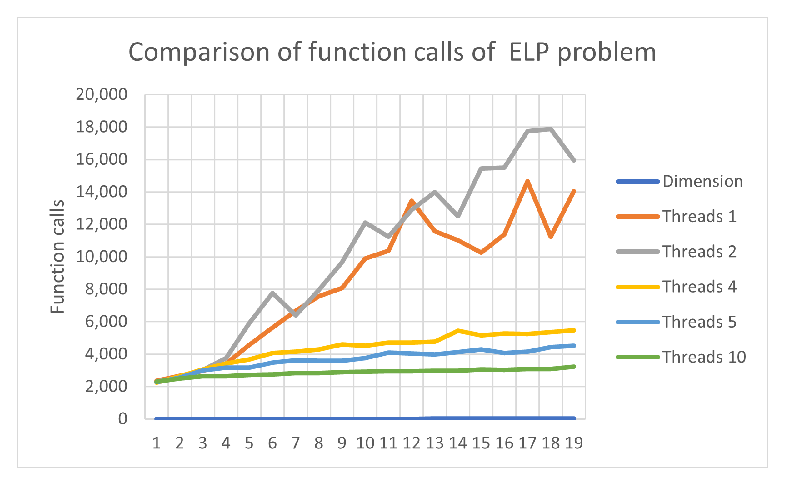
\includegraphics[scale=0.7]{parallelde_scale}

\caption{Scalabilty of the ParallelDe method.\label{fig:Scalability}}
\end{figure}


\subsection{The interface Fuchs-Kliewer polaritons}

Let us consider a double heterostructure made with GaAs/AlAs. The
dielectric functions to describe the interface Fuchs-Kliewer (FK)
polaritons in the heterostructure are given by \cite{fuchss}
\begin{equation}
\epsilon_{i}=\epsilon_{\infty,i}\frac{\omega^{2}-\omega_{L,i}^{2}}{\omega^{2}-\omega_{T,i}^{2}}\label{epsilon}
\end{equation}
where $\epsilon_{\infty,i}$ is the high-frequency dielectric constant,
$\omega_{L,i}$ and $\omega_{L,i}$are the zone center LO and TO optical
frequencies of the i-th material. The symmetric and the antisymmetric
interface mode dispersion relations are respectively given by the
following equations 
\begin{equation}
\frac{\epsilon_{2}(\omega)q_{1}}{\epsilon_{1}(\omega)q_{2}}=-coth(\frac{q_{2}d}{2})\label{disp_S}
\end{equation}

\begin{equation}
\frac{\epsilon_{2}(\omega)q_{1}}{\epsilon_{1}(\omega)q_{2}}=-tanh(\frac{q_{2}d}{2})\label{disp_A}
\end{equation}
The wavevectors $q_{i}$ and the in-plane wavevector $q_{||}$ are
given by 
\begin{equation}
q_{i}^{2}=q_{||}^{2}-\omega^{2}\epsilon_{i}(\omega)/c^{2}\label{wave_vector}
\end{equation}
In the figure \ref{fig:fuchss} by using a genetic algorithm, we present
the two lower interface polariton branches of the double heterostructure
GaAs/AlAs by considering well width d=5 $nm$, $\hbar$ $\omega_{L1}$=50.09
meV, $\hbar$ $\omega_{T1}$=44.88 meV, $\hbar$ $\omega_{L2}$=36.25
meV, $\hbar$ $\omega_{T2}$=33.29 meV, $\epsilon_{\infty,1}$=8.16
and $\epsilon_{\infty,2}$=10.89. The results shown that the proposed
algorithm is very competitive for the studied problem. 

\begin{figure}[H]
\begin{centering}
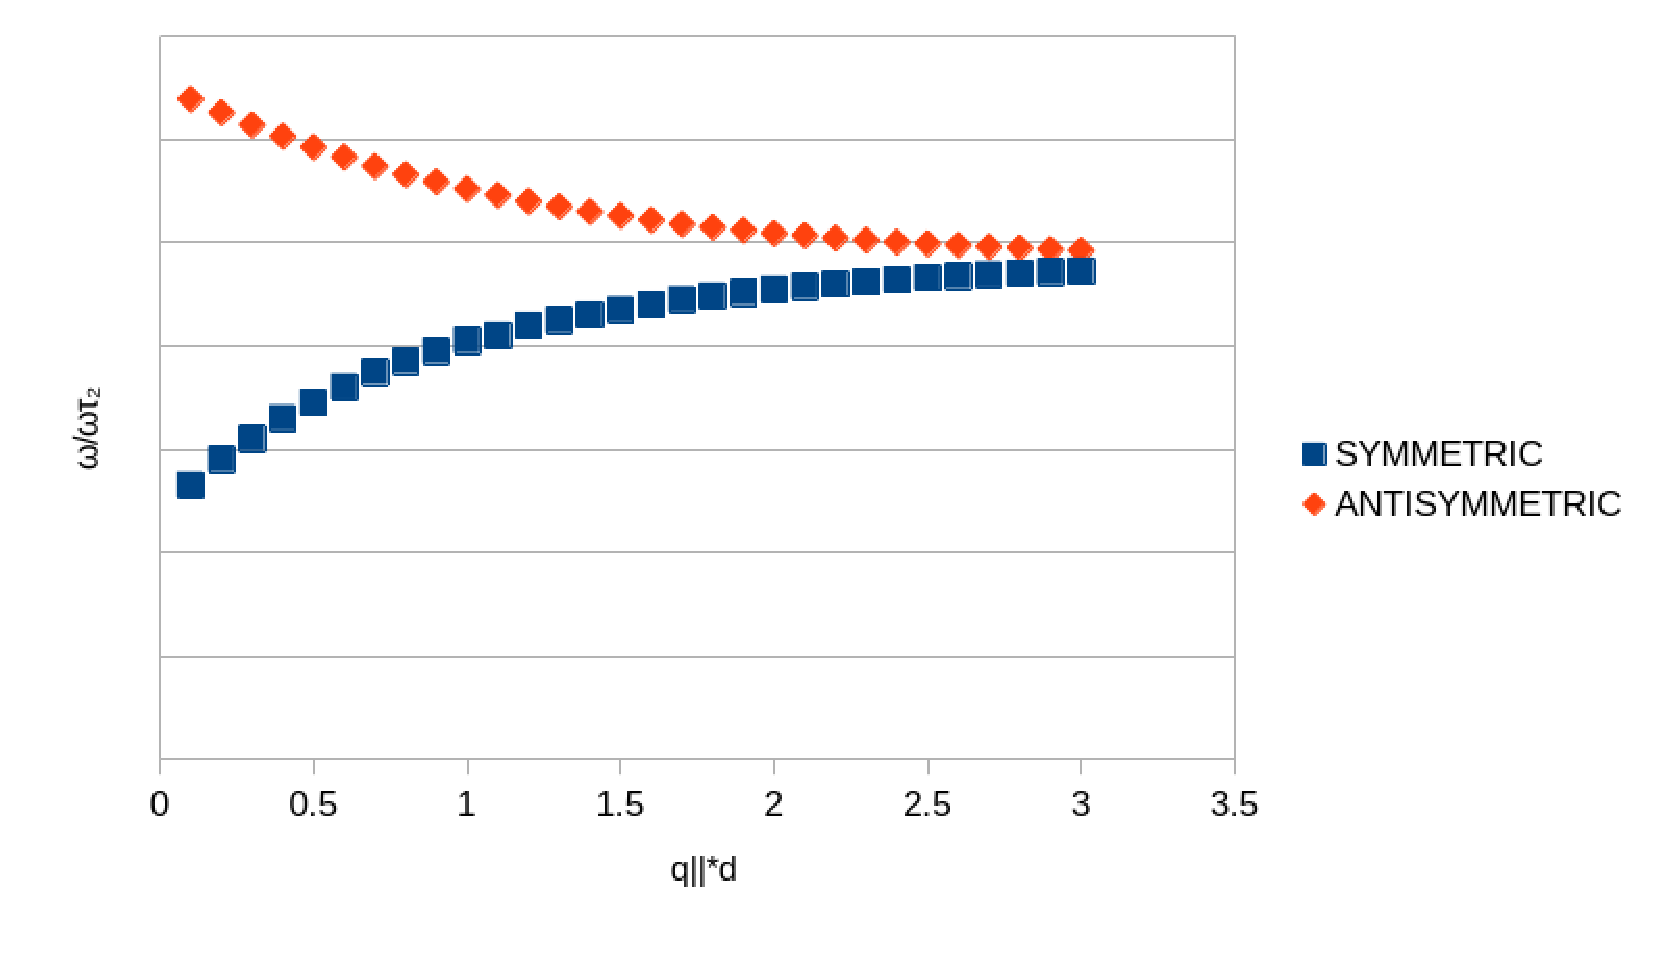
\includegraphics[scale=0.4]{fuchss}
\par\end{centering}
\caption{Using a genetic algorithm for the interface Fuchs-Kliewer polaritons\label{fig:fuchss}}

\end{figure}


\subsection{Experiments with the sampling method}

One more parameter is available for the implemented global minimization
methods of this software package with the name $--$opt\_sampler.
With this parameter, the user can provide an alternative method used
to draw samples from the objective problem. The default value is \emph{uniform},
for the uniform distribution, although the user can use other distributions
such as the triangular distribution \cite{triangular} or use the
K-Means \cite{kmeansNew} to draw samples. An experiment was performed
using the Genetic optimizer and three sampling techniques: uniform,
triangular and K-Means and the results are outlined in Table \ref{tab:sampling}.

\begin{table}[H]

\caption{Experiments with sampling methods using the Genetic optimizer.\label{tab:sampling}}

\centering{}%
\begin{tabular}{|c|c|c|c|}
\hline 
\textbf{PROBLEM} & \textbf{UNIFORM} & \textbf{TRIANGULAR} & \textbf{KMEANS}\tabularnewline
\hline 
\hline 
GRIEWANK2 & 4575 & 3960(0.97) & 2273\tabularnewline
\hline 
GRIEWANK10 & 6542 & 6512 & 5250\tabularnewline
\hline 
EXP32 & 3564 & 3316 & 3471\tabularnewline
\hline 
EXP64 & 3883 & 3612 & 3789\tabularnewline
\hline 
RASTRIGIN & 4358 & 3742 & 2474\tabularnewline
\hline 
SHEKEL5 & 3343 & 3066 & 2081\tabularnewline
\hline 
SHEKEL7 & 3370 & 3124 & 2084\tabularnewline
\hline 
SHEKEL10 & 3496 & 3175 & 2229\tabularnewline
\hline 
TEST2N4 & 3345 & 2968 & 2105\tabularnewline
\hline 
TEST2N5 & 3805 & 3597 & 2551\tabularnewline
\hline 
TEST2N6 & 4299 & 4036 & 2953\tabularnewline
\hline 
TEST2N7 & 4969(0.97) & 4414(0.93) & 3441(0.93)\tabularnewline
\hline 
\textbf{SUM} & \textbf{49549(0.99)} & \textbf{45522(0.99)} & \textbf{34701(0.99)}\tabularnewline
\hline 
\end{tabular}
\end{table}
As can be deduced from the results, the K-Means sampling improves
the speed of the genetic algorithm by reducing the number of function
calls required to obtain the global minimum of any given objective
function in the experiment.

\section{Conclusions\label{sec:Conclusions}}

In this work, an environment for executing global optimization problems
was presented. In this environment, the user can code the objective
problem using some predefined functions and then has the possibility
to choose one among several global optimization methods to solve the
mentioned problem. In addition, it is given the possibility to choose
to use some local optimization method to enhance the reliability of
the produced results. This programming environment is freely available
and easy to extend to accommodate more global optimization techniques.
It is subject to continuous improvements and some of those planned
for the near future are:
\begin{enumerate}
\item Use of modern parallel techniques to speed up the generated results
and implementation of efficient termination techniques. In addition,
new termination techniques specifically designed for parallel techniques
should be devised and implemented.
\item Implementing a GUI interface to control the optimization process.
\item The ability to code the objective function in other programming languages
such as Python, Ada, Fortran etc.
\item Creating a scripting language to efficiently guide the optimization
of objective functions.
\end{enumerate}
\begin{thebibliography}{100}
\bibitem{globalecon1}Zwe-Lee Gaing, Particle swarm optimization to
solving the economic dispatch considering the generator constraints,
IEEE Transactions on \textbf{18} Power Systems, pp. 1187-1195, 2003.

\bibitem{globalecon2}C. D. Maranas, I. P. Androulakis, C. A. Floudas,
A. J. Berger, J. M. Mulvey, Solving long-term financial planning problems
via global optimization, Journal of Economic Dynamics and Control
\textbf{21}, pp. 1405-1425, 1997.

\bibitem{global_physics1}Q. Duan, S. Sorooshian, V. Gupta, Effective
and efficient global optimization for conceptual rainfall-runoff models,
Water Resources Research \textbf{28}, pp. 1015-1031 , 1992.

\bibitem{global_physics2}P. Charbonneau, Genetic Algorithms in Astronomy
and Astrophysics, Astrophysical Journal Supplement \textbf{101}, p.
309, 1995

\bibitem{global_chemistry1}A. Liwo, J. Lee, D.R. Ripoll, J. Pillardy,
H. A. Scheraga, Protein structure prediction by global optimization
of a potential energy function, Biophysics \textbf{96}, pp. 5482-5485,
1999.

\bibitem{global_chemistry2}P.M. Pardalos, D. Shalloway, G. Xue, Optimization
methods for computing global minima of nonconvex potential energy
functions, Journal of Global Optimization \textbf{4}, pp. 117-133,
1994.

\bibitem{global_med1}Eva K. Lee, Large-Scale Optimization-Based Classification
Models in Medicine and Biology, Annals of Biomedical Engineering \textbf{35},
pp 1095-1109, 2007.

\bibitem{global_med2}Y. Cherruault, Global optimization in biology
and medicine, Mathematical and Computer Modelling \textbf{20}, pp.
119-132, 1994.

\bibitem{global_job1}Y. Gao, H. Rong, J.Z. Huang, Adaptive grid job
scheduling with genetic algorithms, Future Generation Computer Systems
\textbf{21}, pp. 151-161, 2005.

\bibitem{global_job2}D.Y. Sha, H.H. Lin, A multi-objective PESO for
job-shop scheduling problems, Expert Systems with Applications \textbf{37},
pp. 1065-1070, 2010.

\bibitem{global_water1}X. Cai, D.C. McKinney, L.S. Lasdon, Solving
nonlinear water management models using a combined genetic algorithm
and linear programming approach, Advances in Water Resources \textbf{24},
pp. 667-676, 2001.

\bibitem{global_water2}S.G. Gino Sophia, V. Ceronmani Sharmila, S.
Suchitra et al, Water management using genetic algorithm-based machine
learning, Soft Comput \textbf{24}, pp. 17153--17165, 2020.

\bibitem{global_network1}Z. Bankovic, D. Stepanovic, S. Bojanic,
O. Nieto - Taladriz, Improving network security using genetic algorithm
approach, Computers \& Electrical Engineering \textbf{33}, pp. 438-451,
2007.

\bibitem{global_network2}S. Paul, I. Dutt, S.N. Choudhri, Design
and implementation of network security using genetic algorithm. Int
J Res Eng Technol \textbf{2}, pp. 172-177, 2013.

\bibitem{global_robot1}A. Tuncer, M. Yildrim, Dynamic path planning
of mobile robots with improved genetic algorithm, Computers \& Electrical
Engineering \textbf{38}, pp. 1564-1572, 2012.

\bibitem{global_robot2}N. Kherici, Y.M. Ben Ali, Using PESO for a
walk of a biped robot, Journal of Computational Science \textbf{5},
pp. 743-749, 2014.

\bibitem{go_symmetry0}B. Freisleben and P. Merz, A genetic local
search algorithm for solving symmetric and asymmetric traveling salesman
problems, In: Proceedings of IEEE International Conference on Evolutionary
Computation, pp. 616-621, 1996.

\bibitem{go_symmetry1}R. Grbi\'{c}, E.K. Nyarko and R. Scitovski,
A modification of the DIRECT method for Lipschitz global optimization
for a symmetric function, J Glob Optim \textbf{57}, pp. 1193--1212,
2013.

\bibitem{go_symmetry2}R. Scitovski, A new global optimization method
for a symmetric Lipschitz continuous function and the application
to searching for a globally optimal partition of a one-dimensional
set, J Glob Optim \textbf{68}, pp. 713--727, 2017.

\bibitem{global_nonlinear1}Barbara Kaltenbacher and William Rundell,
The inverse problem of reconstructing reaction--diffusion systems,
Invese Problems \textbf{36}, 2020.

\bibitem{global_nonlinear2}N. Levashova, A. Gorbachev, R. Argun,
D. Lukyanenko, The Problem of the Non-Uniqueness of the Solution to
the Inverse Problem of Recovering the Symmetric States of a Bistable
Medium with Data on the Position of an Autowave Front., Symmetry \textbf{13},
2021.

\bibitem{global_nonlinear3}Larisa Beilina, Michael V. Klibanov, A
Globally Convergent Numerical Method for a Coefficient Inverse Problem,
SIAM Journal on Scientific Computing \textbf{31},pp. 478-509, 2008. 

\bibitem{go_adaptive1}M. Brunato, R. Battiti, RASH: A Self-adaptive
Random Search Method. In: Cotta, C., Sevaux, M., S�rensen, K. (eds)
Adaptive and Multilevel Metaheuristics. Studies in Computational Intelligence,
vol 136. Springer, Berlin, Heidelberg, 2008.

\bibitem{go_adaptive2}S. Andrad�ttir, A.A. Prudius, A.A., Adaptive
random search for continuous simulation optimization. Naval Research
Logistics \textbf{57}, pp. 583-604, 2010.

\bibitem{go_crs1}W.L. Price, Global optimization by controlled random
search, J Optim Theory Appl \textbf{40}, pp. 333--348, 1983.

\bibitem{go_crs2}P. Kaelo, M.M. Ali, Some Variants of the Controlled
Random Search Algorithm for Global Optimization. J Optim Theory Appl
\textbf{130}, pp. 253--264 (2006).

\bibitem{go_sa1}S. Kirkpatrick, C.D. Gelatt, M.P. Vecchi, Optimization
by simulated annealing, Science \textbf{220}, pp. 671-680, 1983.

\bibitem{go_sa2}K.M.El-Naggar, M.R. AlRashidi, M.F. AlHajri, A.K.
Al-Othman, Simulated Annealing algorithm for photovoltaic parameters
identification, Solar Energy \textbf{86}, pp. 266-274, 2012.

\bibitem{go_sa3}L.M. Rasdi Rere, M.I. Fanany, A.M. Arymurthy, Simulated
Annealing Algorithm for Deep Learning, Procedia Computer Science \textbf{72},
pp. 137-144, 2015.

\bibitem{go_ga1}J. Mc Call, Genetic algorithms for modelling and
optimisation, Journal of Computational and Applied Mathematics \textbf{184},
pp. 205-222, 2005.

\bibitem{go_ga2}C.K.H. Lee, A review of applications of genetic algorithms
in operations management, Elsevier Engineering Applications of Artificial
Intelligence \textbf{76}, pp. 1-12, 2018.

\bibitem{go_ant1}B. Chandra Mohan, R. Baskaran, A survey: Ant Colony
Optimization based recent research and implementation on several engineering
domain, Expert Systems with Applications \textbf{39}, pp. 4618-4627,
2012.

\bibitem{go_ant2}T. Liao, T. St�tzle, M.A. Montes de Oca, M. Dorigo,
A unified ant colony optimization algorithm for continuous optimization,
European Journal of Operational Research \textbf{234}, pp. 597-609,
2014.

\bibitem{go_pso1}D. Wang, D. Tan, L. Liu, Particle swarm optimization
algorithm: an overview. Soft Comput \textbf{22}, pp. 387--408, 2018.

\bibitem{go_pso2}N.K. Jain, U. Nangia, J. Jain, A Review of Particle
Swarm Optimization. J. Inst. Eng. India Ser. B \textbf{99}, pp. 407--411,
2018.

\bibitem{go_pso_genetic_hybrid1}D.H. Kim, A. Abraham, J.H. Cho, A
hybrid genetic algorithm and bacterial foraging approach for global
optimization, Information Sciences \textbf{177}, pp. 3918-3937, 2007.

\bibitem{go_pso_genetic_hybrid2}Y.T. Kao, E. Zahara, A hybrid genetic
algorithm and particle swarm optimization for multimodal functions,
Applied Soft Computing \textbf{8}, pp. 849-857, 2008.

\bibitem{ga_fuzzy}G.T. Reddy, M.P.K. Reddy, K. Lakshmanna et al,
Hybrid genetic algorithm and a fuzzy logic classifier for heart disease
diagnosis, Evol. Intel. \textbf{13}, pp. 185--196, 2020.

\bibitem{ga_kmeans}M.D. Anisur Rahman, M.D. Zahidul Islam, A hybrid
clustering technique combining a novel genetic algorithm with K-Means,
Knowledge-Based Systems \textbf{71}, pp. 345-365, 2014.

\bibitem{pso_aco1}T. Niknam, An efficient hybrid evolutionary algorithm
based on PESO and ACO for distribution feeder reconfiguration, European
Transactions on Electrical Power \textbf{20}, pp. 575-590, 2010.

\bibitem{pso_aco2}M.K. Patel, M.R. Kabat, C.R. Tripathy, A hybrid
ACO/PESO based algorithm for QoS multicast routing problem, Ain Shams
Engineering Journal \textbf{5}, pp. 113-120, 2014.

\bibitem{pso_aco3}A.K. Dubey, A. Kumar, R. Agrawal, An efficient
ACO-PSO-based framework for data classification and preprocessing
in big data, Evol. Intel. \textbf{14}, pp. 909--922, 2021.

\bibitem{hybrid1}Offord C., Bajzer �. (2001) A Hybrid Global Optimization
Algorithm Involving Simplex and Inductive Search. In: Alexandrov V.N.,
Dongarra J.J., Juliano B.A., Renner R.S., Tan C.J.K. (eds) Computational
Science - ICCS 2001. ICCS 2001. Lecture Notes in Computer Science,
vol 2074. Springer, Berlin, Heidelberg.

\bibitem{go_local1}S. Li, M. Tan, I. W. Tsang, J. T. -Y. Kwok, A
Hybrid PSO-BFGS Strategy for Global Optimization of Multimodal Functions,
IEEE Transactions on Systems, Man, and Cybernetics, Part B (Cybernetics)
\textbf{41}, pp. 1003-1014, 2011.

\bibitem{go_local2}H. Badem, A. Basturk, A. Caliskan, M.E. Yuksel,
A new hybrid optimization method combining artificial bee colony and
limited-memory BFGS algorithms for efficient numerical optimization,
Applied Soft Computing \textbf{70}, pp. 826-844, 2018.

\bibitem{go_local3}A.A. Nagra, F. Han, Q.H. Ling, An improved hybrid
self-inertia weight adaptive particle swarm optimization algorithm
with local search, Engineering Optimization \textbf{51}, pp. 1115-1132,
2018.

\bibitem{genetic_physics1}S.Q. Wu, M. Ji, C.Z. Wang, M.C. Nguyen,
X. Zhao, K. Umemoto, R. M. Wentzcovitch, K. M. Ho, An adaptive genetic
algorithm for crystal structure prediction, Journal of Physics: Condensed
Matter \textbf{26}, 035402, 2013.

\bibitem{genetic_physics2}M. Honda, Application of genetic algorithms
to modelings of fusion plasma physics, Computer Physics Communications
\textbf{231}, pp. 94-106, 2018.

\bibitem{genetic_physics3}X.L. Luo, J. Feng, H.H. Zhang, A genetic
algorithm for astroparticle physics studies, Computer Physics Communications
\textbf{250}, 106818, 2020.

\bibitem{pso_physics1}M. Ye, X. Wang, Y. Xu, Parameter extraction
of solar cells using particle swarm optimization, Journal of Applied
Physics \textbf{105}, 094502. 2009.

\bibitem{pso_physics2}A. Belkadi, L. Ciarletta, D. Theilliol, Particle
swarm optimization method for the control of a fleet of Unmanned Aerial
Vehicles, Journal of Physics: Conference Series, Volume 659, 12th
European Workshop on Advanced Control and Diagnosis (ACD 2015) 19--20
November 2015, Pilsen, Czech Republic.

\bibitem{async1}M. Depolli, R. Trobec, B. Filipi\v{c}, Asynchronous
Master-Slave Parallelization of Differential Evolution for Multi-Objective
Optimization, Evolutionary Computation \textbf{21}, pp. 261-291, 2013.

\bibitem{async2}A. P. Engelbrecht, Asynchronous particle swarm optimization
with discrete crossover, In: 2014 IEEE Symposium on Swarm Intelligence,
Orlando, FL, USA, 2014, pp. 1-8.

\bibitem{async3}F. Bourennani, Cooperative asynchronous parallel
particle swarm optimization for large dimensional problems, International
Journal of Applied Metaheuristic Computing (IJAMC) \textbf{10.3},
pp. 19-38, 2019.

\bibitem{parallel-multistart}J. Larson and S.M. Wild, Asynchronously
parallel optimization solver for finding multiple minima, Mathematical
Programming Computation \textbf{10}, pp. 303-332, 2018.

\bibitem{parallel-multistart2}H.P.J. Bolton, J.F. Schutte, A.A. Groenwold,
Multiple Parallel Local Searches in Global Optimization. In: Dongarra
J., Kacsuk P., Podhorszki N. (eds) Recent Advances in Parallel Virtual
Machine and Message Passing Interface. EuroPVM/MPI 2000. Lecture Notes
in Computer Science, vol 1908. Springer, Berlin, Heidelberg, 2000.

\bibitem{gpu1}Y. Zhou and Y. Tan, GPU-based parallel particle swarm
optimization, In: 2009 IEEE Congress on Evolutionary Computation,
2009, pp. 1493-1500.

\bibitem{gpu2}L. Dawson and I. Stewart, Improving Ant Colony Optimization
performance on the GPU using CUDA, In: 2013 IEEE Congress on Evolutionary
Computation, 2013, pp. 1901-1908.

\bibitem{gpu3}Barkalov, K., Gergel, V. Parallel global optimization
on GPU. J Glob Optim \textbf{66}, pp. 3--20, 2016.

\bibitem{baron}N.V. Sahinidis, BARON: A general purpose global optimization
software package, J Glob Optim \textbf{8}, pp. 201--205, 1996.

\bibitem{merlin}D.G. Papageorgiou, I.N. Demetropoulos, I.E. Lagaris,
Computer Physics Communications \textbf{159}, pp. 70-71, 2004.

\bibitem{deoptim}K. Mullen, D. Ardia, D.L. Gil, D. Windover, J. Cline,
DEoptim: An R Package for Global Optimization by Differential Evolution,
Journal of Statistical Software \textbf{40}, pp. 1-26, 2011.

\bibitem{pdoublepop}I.G. Tsoulos, A. Tzallas, D. Tsalikakis, PDoublePop:
An implementation of parallel genetic algorithm for function optimization,
Computer Physics Communications \textbf{209}, pp. 183-189, 2016.

\bibitem{paradiseo}J. Dreo, A. Liefooghe, S. Verel, M. Schoenauer,
J.J. Merelo, A. Quemy, B. Bouvier, J. Gmys, Paradiseo: from a modular
framework for evolutionary computation to the automated design of
metaheuristics ---22 years of Paradiseo---, GECCO'21: Proceedings
of the Genetic and Evolutionary Computation Conference Companion,
1522--1530, 2021.

\bibitem{pagmo}F. Biscani, D. Izzo, A parallel global multiobjective
framework for optimization: pagmo, Journal of Open Source Software
\textbf{5}, 2338, 2020.

\bibitem{de_main_paper}R. Storn, On the usage of differential evolution
for function optimization, In: Proceedings of North American Fuzzy
Information Processing, pp. 519-523, 1996.

\bibitem{de_datamining}I. Triguero, S. Garcia, F. Herrera, Differential
evolution for optimizing the positioning of prototypes in nearest
neighbor classification, Pattern Recognition \textbf{44}, pp. 901-916,
2011.

\bibitem{de_symmetry1}Y.H. Li, J.Q. Wang, X.J. Wang, Y.L. Zhao, X.H.
Lu, D.L. Liu, Community Detection Based on Differential Evolution
Using Social Spider Optimization, Symmetry \textbf{9}, 2017.

\bibitem{de_symmetry3}W. Yang, E.M. Dilanga Siriwardane, R. Dong,
Y. Li, J. Hu, Crystal structure prediction of materials with high
symmetry using differential evolution, J. Phys.: Condens. Matter \textbf{33}
455902, 2021.

\bibitem{de_symmetry6}C.Y. Lee, C.H. Hung, Feature Ranking and Differential
Evolution for Feature Selection in Brushless DC Motor Fault Diagnosis
, Symmetry \textbf{13}, 2021.

\bibitem{de_symmetry7}S. Saha, R. Das, Exploring differential evolution
and particle swarm optimization to develop some symmetry-based automatic
clustering techniques: application to gene clustering, Neural Comput
\& Applic \textbf{30}, pp. 735--757, 2018.

\bibitem{parallelDe}V. Charilogis, I.G. Tsoulos, A Parallel Implementation
of the Differential Evolution Method, Analytics \textbf{2}, pp. 17-30,
2023.

\bibitem{openMp}R. Chandra, L. Dagum, D. Kohr, D. Maydan,J. McDonald
and R. Menon, Parallel Programming in OpenMP, Morgan Kaufmann Publishers
Inc., 2001.

\bibitem{doublepop_tsoulos}I.G. Tsoulos, Modifications of real code
genetic algorithm for global optimization, Applied Mathematics and
Computation \textbf{203}, pp. 598-607, 2008.

\bibitem{genetic1}J.F.Gon�alves, J.J.M. Mendes, M.G.C. Resende, A
genetic algorithm for the resource constrained multi-project scheduling
problem, European Journal of Operational Research \textbf{189}, pp.
1171-1190, 2008.

\bibitem{genetic2}W.Ho, G.T.S. Ho, P. Ji, H.C.W. Lau, A hybrid genetic
algorithm for the multi-depot vehicle routing problem, Engineering
Applications of Artificial Intelligence \textbf{21}, pp. 548-557,
2008.

\bibitem{genetic3}J.F. Gon�alves, M.G.C. Resende, Biased random-key
genetic algorithms for combinatorial optimization. J Heuristics \textbf{17},
pp. 487--525, 2011.

\bibitem{genetic4}M. Turrin, P. Buelow, R. Stouffs, Design explorations
of performance driven geometry in architectural design using parametric
modeling and genetic algorithms, Advanced Engineering Informatics
\textbf{25}, pp. 656-675, 2011.

\bibitem{psoApp1}M. Ye, X. Wang, Y. Xu, Parameter extraction of solar
cells using particle swarm optimization, Journal of Applied Physics
\textbf{105}, 094502, 2009.

\bibitem{psoApp2}Y. Wang, J. Lv, L. Zhu, Y. Ma, Crystal structure
prediction via particle-swarm optimization, Phys. Rev. B \textbf{82},
094116, 2010.

\bibitem{psoApp3}M. Weiel, M. G�tz, A. Klein et al, Dynamic particle
swarm optimization of biomolecular simulation parameters with flexible
objective functions. Nat Mach Intell \textbf{3}, pp. 727--734, 2021.

\bibitem{ipso}V. Charilogis, I.G. Tsoulos, Toward an Ideal Particle
Swarm Optimizer for Multidimensional Functions, Information \textbf{13},
217, 2022.

\bibitem{multistart-tsp}Li W., A Parallel Multi-start Search Algorithm
for Dynamic Traveling Salesman Problem. In: Pardalos P.M., Rebennack
S. (eds) Experimental Algorithms. SEA 2011. Lecture Notes in Computer
Science, vol 6630. Springer, Berlin, Heidelberg, 2011.

\bibitem{multistart-vehicle}Olli Br�ysy, Geir Hasle, Wout Dullaert,
A multi-start local search algorithm for the vehicle routing problem
with time windows, European Journal of Operational Research \textbf{159},
pp. 586-605, 2004.

\bibitem{multistart_fac}Mauricio G.C. Resende, Renato F. Werneck,A
hybrid multistart heuristic for the uncapacitated facility location
problem, European Journal of Operational Research \textbf{174}, pp.
54-68, 2006.

\bibitem{multistart_clique}E. Marchiori, Genetic, Iterated and Multistart
Local Search for the Maximum Clique Problem. In: Cagnoni S., Gottlieb
J., Hart E., Middendorf M., Raidl G.R. (eds) Applications of Evolutionary
Computing. EvoWorkshops 2002. Lecture Notes in Computer Science, vol
2279. Springer, Berlin, Heidelberg. 

\bibitem{multistart_fire}Gomes M.I., Afonso L.B., Chibeles-Martins
N., Fradinho J.M. (2018) Multi-start Local Search Procedure for the
Maximum Fire Risk Insured Capital Problem. In: Lee J., Rinaldi G.,
Mahjoub A. (eds) Combinatorial Optimization. ISCO 2018. Lecture Notes
in Computer Science, vol 10856. Springer, Cham. https://doi.org/10.1007/978-3-319-96151-4\_19

\bibitem{multistart-aero}Streuber, Gregg M. and Zingg, David. W.,
Evaluating the Risk of Local Optima in Aerodynamic Shape Optimization,
AIAA Journal 59, pp. 75-87, 2012.

\bibitem{rbf_main1}J. Park, I.W. Sandberg, Approximation and Radial-Basis-Function
Networks, Neural Computation \textbf{5}, pp. 305-316, 1993.

\bibitem{neuralMinimizer}I.G. Tsoulos, A. Tzallas, E. Karvounis,
D. Tsalikakis, NeuralMinimizer, a novel method for global optimization
that incorporates machine learning, Information \textbf{14}, 2, 2023.

\bibitem{ppso}V. Charilogis, I.G. Tsoulos, A. Tzallas, An Improved
Parallel Particle Swarm Optimization, SN COMPUT. SCI. \textbf{4},
766, 2023.

\bibitem{corana}A. Corana, M. Marchesi, C. Martini, S. Ridella, Minimizing
multimodal functions of continuous variables with the \textquotedblleft Simulated
Annealing\textquotedblright{} algo- rithm, ACM Trans. Math. Software
\textbf{13}, pp. 262--280, 1987.

\bibitem{powell}M.J.D Powell, A Tolerant Algorithm for Linearly Constrained
Optimization Calculations, Mathematical Programming \textbf{45}, pp.
547-566, 1989. 

\bibitem{lbfgs}D.C. Liu, J. Nocedal, On the Limited Memory Method
for Large Scale Optimization, Mathematical Programming B \textbf{45},
pp. 503-528, 1989.

\bibitem{gradient1}S.I. Amari, Backpropagation and stochastic gradient
descent method, Neurocomputing \textbf{5}, pp. 185-196, 1993.

\bibitem{gradient2}S. Klein, J.P.W. Pluim, M. Staring, Adaptive Stochastic
Gradient Descent Optimisation for Image Registration, Int J Comput
Vis \textbf{81}, pp. 227--239, 2009.

\bibitem{nelderMead}D.M. Olsson,L.S. Nelson, The Nelder-Mead Simplex
Procedure for Function Minimization, Technometrics \textbf{17}, pp.
45-51, 1975.

\bibitem{Adam}D.P. Kingma, J. Ba, Adam: A Method for Stochastic Optimization,
ICLR (Poster), 2015.

\bibitem{adept}R.J. Hogan, Fast reverse-mode automatic differentiation
using expression templates in C++. ACM Trans. Math. Softw. \textbf{40},
pp. 1-26, 2014.

\bibitem{originalJones}J.E. Lennard-Jones, On the Determination of
Molecular Fields, Proc. R. Soc. Lond. A \textbf{ 106}, pp. 463--477,
1924.

\bibitem{nn1}C. Bishop, Neural Networks for Pattern Recognition,
Oxford University Press, 1995.

\bibitem{nn2}G. Cybenko, Approximation by superpositions of a sigmoidal
function, Mathematics of Control Signals and Systems \textbf{2}, pp.
303-314, 1989.

\bibitem{testfunctions1}M.M. Ali and P. Kaelo, Improved particle
swarm algorithms for global optimization, Applied Mathematics and
Computation \textbf{196}, pp. 578-593, 2008.

\bibitem{testfunctions2}H. Koyuncu, R. Ceylan, A PESO based approach:
Scout particle swarm algorithm for continuous global optimization
problems, Journal of Computational Design and Engineering \textbf{6},
pp. 129--142, 2019.

\bibitem{testfunctions3}Patrick Siarry, G�rard Berthiau, Fran�ois
Durdin, Jacques Haussy, ACM Transactions on Mathematical Software
\textbf{23}, pp 209--228, 1997.

\bibitem{testfunctions4}I.G. Tsoulos, I.E. Lagaris, GenMin: An enhanced
genetic algorithm for global optimization, Computer Physics Communications\textbf{
178, }pp. 843-851, 2008.

\bibitem{Jones}J.A. Northby, Structure and binding of Lennard-Jones
clusters: 13 \ensuremath{\le} n \ensuremath{\le} 147, J. Chem. Phys.
\textbf{87}, pp. 6166--6178, 1987.

\bibitem{fuchss} B. K. Ridley, Electrons and Phonons in Semiconductor
Multilayers, Cambridge University Press, 2nd edition (2014) 

\bibitem{jonesNew}G.L. Xue, R.S. Maier, J.B. Rosen, Improvements
on the Northby Algorithm for molecular conformation: Better solutions,
J. Global. Optim. 4, pp. 425--440, 1994.

\bibitem{triangular}W.E. Stein, M.F. Keblis, A new method to simulate
the triangular distribution, Mathematical and Computer Modelling Volume
\textbf{49}, pp. 1143-1147, 2009.

\bibitem{kmeansNew}M. Ahmed, R. Seraj, S.M.S. Islam, The k-means
algorithm: A comprehensive survey and performance evaluation, Electronics
\textbf{9}, 1295, 2020.

\end{thebibliography}

\end{document}
